\documentclass[tikz,border=2pt]{standalone}
\usepackage{tikz}
\usetikzlibrary{arrows.meta,positioning,fit,shapes.geometric}
\begin{document}
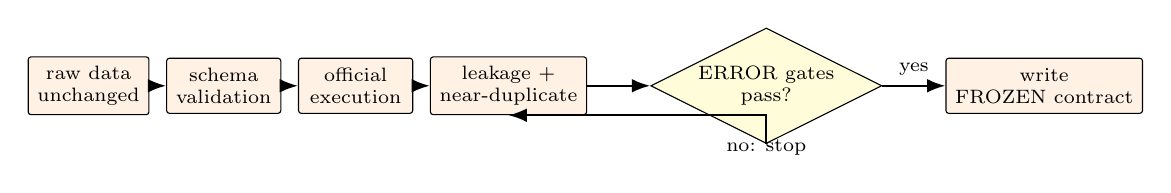
\begin{tikzpicture}[node distance=4pt and 6pt, >=Latex,
  gstep/.style={draw, rounded corners=1pt, fill=orange!10, align=center,
    minimum width=1.45cm, minimum height=0.7cm, font=\scriptsize},
  decision/.style={draw, diamond, aspect=2.0, fill=yellow!15, align=center,
    inner sep=1pt, font=\scriptsize}, arrow/.style={->, thick}]
\node[gstep] (raw) {raw data\\unchanged};
\node[gstep, right=of raw] (schema) {schema\\validation};
\node[gstep, right=of schema] (exec) {official\\execution};
\node[gstep, right=of exec] (leak) {leakage +\\near-duplicate};
\node[decision, right=8mm of leak] (pass) {ERROR gates\\pass?};
\node[gstep, right=8mm of pass] (freeze) {write\\FROZEN contract};
\draw[arrow] (raw) -- (schema);
\draw[arrow] (schema) -- (exec);
\draw[arrow] (exec) -- (leak);
\draw[arrow] (leak) -- (pass);
\draw[arrow] (pass) -- node[above, font=\scriptsize]{yes} (freeze);
\draw[arrow] (pass.south) |- node[pos=0.25, below, font=\scriptsize]{no: stop} (leak.south);
\end{tikzpicture}
\end{document}
